\subsection{L2: Autonomy over Improvement Strategies}
\label{sec:l2-strategy}

At L2, the AI system uses evaluation feedback to choose which improvement
intervention to attempt next, rather than merely executing a prescribed
update.
It proposes and tests changes to the target and retains accepted
revisions, while humans continue to specify the objective, task boundary, and acceptance criteria.
The surrounding search framework may remain fixed; autonomy lies in determining how the target should be improved.
In many AI-development workflows, executing a proposed change is comparatively mechanical; the difficult part is deciding which change is worth trying. Researchers must interpret failures, infer which component is limiting progress, choose an intervention whose effect is uncertain, and decide what to try next after observing the result. As the space of possible interventions grows, this experimental decision-making becomes a major bottleneck: exhaustive search is infeasible, while manual experimentation is constrained by researcher attention and prior intuitions.
L2 systems automate this bottleneck. Rather than merely carrying out a human-specified modification, the \Improver \ uses evaluation results and experimental evidence to determine the next candidate intervention.

This transition increasingly resembles partial automation of the empirical researcher's role. OpenAI, for example, describes current frontier agents as reaching an ``automated research intern'' stage for well-defined research tasks under human supervision, while researchers continue to set priorities and decide which results merit further investment or deployment~\cite{openai2026researchacceleration}. The relevant autonomy is therefore not unrestricted control of research, but the transfer of a specific research responsibility: turning observed evidence into the next experiment.

The characteristic loop at this level can be summarized as follows:
% $$
% \begin{aligned}
% &\textit{observe performance}
% \rightarrow
% \textit{diagnose}
% \\
% &\rightarrow
% \textit{select how change}
% \rightarrow
% \textit{instantiate and test}\\
% &
% \rightarrow
% \textit{retain or revert}
% \rightarrow
% \textit{repeat}.
% \end{aligned}
% $$
\begin{center}
\fcolorbox{black!25}{gray!4}{%
\begin{minipage}{0.72\linewidth}
\centering
\vspace{6pt}

\LoneStep{observe performance}
\(\;\longrightarrow\;\)
\LoneStep{diagnose}
\(\;\longrightarrow\;\)
\LoneStep{select how change}

\vspace{7pt}

\(\;\longrightarrow\;\)
\LoneStep{instantiate and test}
\(\;\longrightarrow\;\)
\LoneStep{retain or revert}
\(\;\longrightarrow\;\)
\LoneStep{repeat}

\vspace{6pt}
\end{minipage}%
}
\end{center}

The object being improved may remain small, as in prompt optimization, or expand to an executable agent and eventually to a model-training program. What changes across these settings is the object and scope of intervention available to the improver, together with the evidence available for deciding which modification to attempt. We therefore organize L2 by the \emph{object over which improvement strategies are searched}, rather than by individual systems.
Figure~\ref{fig:L2} illustrates this
strategy-autonomy mechanism, in which evidence about the current system
guides the autonomous selection and evaluation of how to improve it.


\begin{figure*}[!t]
    \centering
    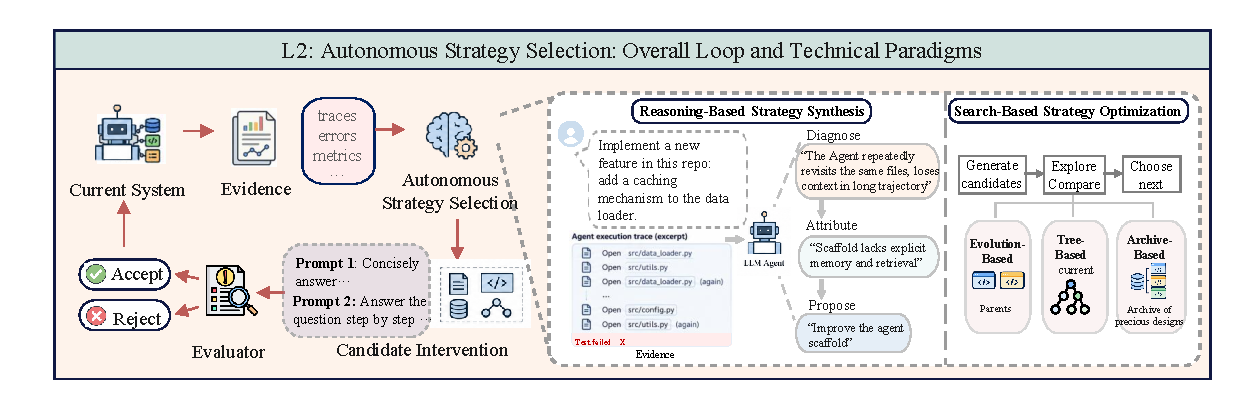
\includegraphics[width=1\linewidth]{figures/L2-v2.pdf}
    \caption{Overview of L2: Autonomous Strategy Selection. Under human-defined improvement objectives and evaluation criteria, the AI system uses evidence from the current system to diagnose weaknesses and autonomously determine how to improve it. Candidate interventions are evaluated, and accepted updates are incorporated into subsequent iterations. Representative mechanisms include reasoning-based strategy synthesis and search-based strategy optimization.}
    \label{fig:L2}
\end{figure*}

% \subsubsection{Language-Level Strategy Search}
\subsubsection{Prompt Search}
\noindent\textbf{The \Improver \ decides how the instructions that govern a model or agent should be changed based on execution traces and evaluation results.} In the narrowest L2 setting, the system decides how a prompt or textual control variable should be revised rather than merely instantiating a prescribed edit. For example, Dropbox used GEPA to rewrite the prompt that tells an LLM how to judge whether retrieved files or messages are relevant to a user's search~\cite{dropbox2026dspy}.
However, earlier evolutionary methods search over alternative mutations, while more recent reflective optimizers use execution traces to identify failure modes and generate targeted revisions. GEPA attributes failures to particular modules and preserves complementary prompt variants rather than committing immediately to a single greedy lineage~\cite{agrawal2026gepa}. This feedback-driven search is not restricted to a single optimizer design. MPO extends the editable surface to multimodal prompts, using evaluation-derived semantic feedback to guide subsequent textual and non-textual prompt candidates, while C-Evolve embeds candidate generation within a fixed evolutionary protocol. Across these settings, the search machinery can be externally specified while the concrete prompt revisions emerge from evaluation feedback.~\cite{choi2026mpo,li2026cevolve}.
The relevant increase in autonomy is therefore not prompt generation itself, but control over which revision strategy is attempted next.


\subsubsection{Agent and Harness Search}
\noindent\textbf{Improvement can involve redesigning how reasoning and tool-using components interact.} Once the editable object expands from a prompt to executable agent code, strategy search begins to resemble automated system design.  % 开宗明义
For example, Microsoft Foundry's Agent Optimizer rewrites hosted agents' system instructions, skills, and local function-tool descriptions from evaluation failures~\cite{microsoft2026agentoptimizer}.
Automated Design of Agentic Systems (ADAS) formalizes an agent as a Python \texttt{forward} function and uses a meta-agent to populate an ever-growing archive of candidate agents~\cite{hu2025adas}. In each iteration, the meta-agent evaluates the candidate on validation data and stores both its code and metrics in the archive.
% The search can therefore modify prompts, role assignments, tool calls, control flow, and feedback loops jointly rather than treating them as independently tuned components. 
Because these decisions are encoded in executable harness code, a single revision can change how the agent behaves throughout an entire task rather than only changing one instruction.


Recent workflow-search systems instantiate this idea through different representations of the design space. 
AFlow encodes workflows as executable graphs and applies Monte Carlo tree search to successive code-level modifications, using execution outcomes as feedback for later branches~\cite{zhang2025aflow}.
AgentSquare instead factorizes agent designs into reusable modules and searches through evolution and recombination, allowing successful structures discovered in one configuration to become building blocks for another~\cite{shang2025agentsquare}.


The resulting autonomy is substantially greater than local parameter tuning while remaining bounded in an important sense. The improver chooses among alternative agent designs, yet candidates are still promoted because they perform better under an externally maintained evaluation process. L2 autonomy concerns the search for a better system configuration; it does not imply authority to redefine what constitutes successful performance.



\subsubsection{Model and Training Search}
\noindent\textbf{The \Improver \ converts empirical training evidence into decisions about how the learner itself should be configured, structured, or optimized.}
Human researchers therefore rely heavily on accumulated intuition to decide which small fraction of the possible experiments to run. The emerging role of an L2 improver is to compress this experimental cycle: inspect what happened in previous runs, infer where improvement is likely to come from, and allocate the next experiment accordingly. Current systems increasingly search over persistent configurations, model structure, and the learning procedure itself.

\noindent$\bullet$ \underline{(1) {Configuration Search.}}
{It automates the allocation of expensive training trials. }% when good settings depend on interacting model, data, and compute conditions.}
Recent agentic approaches increasingly augment conventional search with semantic reasoning about previous experiments. Rather than treating each trial as an isolated black-box query, the system can interpret training outcomes and use them to concentrate subsequent exploration. For example, NVIDIA's 2026 TAO workflow for post-training Cosmos 3 lets a coding agent invoke LLM-guided AutoML under a fixed validation objective~\cite{nvidia2026taoautoml}.
The human supplies the model, task, data, and desired metric; the system takes over much of the repeated decision of which configuration should be evaluated next.

\noindent$\bullet$ \underline{(2) {Architecture Search.}}
It delegates the structural design of the model, reducing reliance on a human-engineered search space.
LLM-based improvers can interpret empirical results and propose structural changes whose exact content was not enumerated beforehand. %\dyemf{OpenAI reports that GPT-5.6 Sol used this capability to improve its own speculative-decoding draft model. Instead of being given a fixed architecture sweep, the model designed and ran hundreds of experiments over changes to the draft model's size, structure, and features, while also monitoring the associated training runs.~\cite{openai2026gpt56efficiency}.}
AgentNAS starts from the observation that modern NAS still depends on manually engineered, task-specific search spaces. It uses an LLM to produce a task-specific seed architecture and then derives a structured search space from that design for subsequent combinatorial search~\cite{jeong2026agentnas}.


\noindent$\bullet$ \underline{(3) {Training-Rule Search.}}
The \Improver\ changes the executable procedure by which model parameters are learned.
Current frontier agents are beginning to automate this hypothesis-to-experiment step. OpenAI's NanoGPT evaluation for GPT-6 Astra gives the agent a fixed validation target, one GPU, and a constrained training setup, but requires the agent itself to diagnose training bottlenecks, modify the training code, tune its configuration, and make useful changes to the training loop~\cite{openai2026gpt6astra}.
Open research environments expose the same division of labor more directly. In \texttt{autoresearch}, the data pipeline, evaluation function, metric, and per-experiment compute budget remain fixed, while the agent repeatedly edits the training program and keeps a modification only when the protected validation metric improves~\cite{karpathy2026autoresearch}.

\noindent$\bullet$ \underline{(4) {Systems and Implementation Search.}}
The \Improver \ searches for a more efficient realization of a model's computation while correctness and system-level performance remain protected by external tests.
AI can profile a bottleneck, propose an implementation change, verify numerical correctness, measure real hardware performance, and use the result to decide what to modify next.
AutoKernel begins from profiling rather than arbitrary code generation: it identifies operations with the largest potential end-to-end impact and directs the agent's experiments toward those bottlenecks. Candidate Triton or CUDA implementations are accepted only after correctness checks and measured GPU speedups~\cite{jaber2026autokernel}.


Table~\ref{tab:l2-strategy-summary} compares representative systems by their search target, mechanism, and externally fixed limitation.

\begin{table*}[t]
\centering
\caption{Representative (rather than exhaustive) L2 systems grouped by the object of improvement-strategy search. All listed systems remain at L2 because they autonomously choose how to improve the system while the objective, evaluation criterion, or acceptance rule remains externally specified.}
\label{tab:l2-strategy-summary}
\scriptsize
\setlength{\tabcolsep}{1.2pt}
\renewcommand{\arraystretch}{1.05}
\begin{tabularx}{0.9\textwidth}{@{}>{\raggedright\arraybackslash}p{0.205\textwidth}>{\raggedright\arraybackslash}p{0.195\textwidth}>{\raggedright\arraybackslash}p{0.3\textwidth}>{\raggedright\arraybackslash}X@{}}
\toprule
\textbf{Method} 
& \textbf{Type} 
& \textbf{Key mechanism} 
& \textbf{Level limitation}\\

\midrule
\multicolumn{4}{@{}l}{\textbf{Prompt Search}}\\

Promptbreeder~\cite{fernando2024promptbreeder}
& Prompt search
& Prompt and mutation co-evolution
& Fixed task fitness \\

GEPA~\cite{agrawal2026gepa}
& Prompt search
& Trace reflection + Pareto selection
& Fixed task metric \\

MPO~\cite{choi2026mpo}
& Prompt search (multimodal)
& Evaluation-derived semantic feedback guides textual and non-textual prompt candidates
& Fixed task metric \\

C-Evolve~\cite{li2026cevolve}
& Prompt search
& Candidate generation inside a fixed evolutionary protocol
& Fixed protocol + task metric \\

\midrule

\multicolumn{4}{@{}l}{\textbf{Agent and Harness Search}}\\
Microsoft Foundry Agent Optimizer~\cite{microsoft2026agentoptimizer}
& Agent search
& Rewrites system instructions, skills, and local function-tool descriptions from evaluation failures
& Fixed evaluation process \\

ADAS~\cite{hu2025adas}
& Agent search
& Meta-agent coding + design archive
& Fixed benchmark \\

AFlow~\cite{zhang2025aflow}
& Workflow search
& MCTS over executable workflows
& Fixed evaluator \\

AgentSquare~\cite{shang2025agentsquare}
& Agent search
& Module evolution + recombination
& Fixed benchmark \\
\midrule

\multicolumn{4}{@{}l}{\textbf{Autonomous Experimental Search}}\\

AutoResearch~\cite{karpathy2026autoresearch}
& ML experiment
& Edit--train--evaluate loop
& Fixed metric \\

GPT-6 Astra NanoGPT~\cite{openai2026gpt6astra}
& Training-rule search
& Agent diagnoses bottlenecks, edits training code, tunes configuration and training loop
& Fixed validation target + compute \\

Auto Research~\cite{ning2026autoresearch}
& ML experiment
& Specialist agents + shared lineage
& External evaluator \\

AgentNAS~\cite{jeong2026agentnas}
& Architecture search
& LLM-generated task-specific seed architecture + derived structured search space
& Fixed validation metric \\

AutoKernel~\cite{jaber2026autokernel}
& Kernel experiment
& Profile--rewrite--benchmark loop
& Fixed correctness + speed \\

% GPT-5.6 Sol~\cite{openai2026gpt56efficiency}
% & Kernel experiment
% & Kernel rewrite + validation
% & Fixed correctness + speed \\
\bottomrule
\end{tabularx}
\end{table*}


\subsubsection{Evaluating L2 Strategy Autonomy}
Greater autonomy over improvement strategy does not by itself imply stronger recursive self-improvement. An L2 system may have a very expressive intervention space and nevertheless search it inefficiently, exploit weaknesses in its evaluator, or produce gains that disappear after several iterations. We therefore separate the \emph{degree of delegated autonomy} from the \emph{quality of the resulting improvement process}.

These dimensions are complementary: a broader search space is useful only if feedback can discriminate among candidates and the search process can explore that space efficiently. This combination helps explain why current industrial systems concentrate on coding, model training, and kernel optimization, where candidate interventions are executable and feedback can be obtained rapidly.

The same adaptive search loop also creates characteristic evaluation hazards. Repeated development-set access invites benchmark overfitting, additional search compute can be mistaken for algorithmic improvement, and an LLM evaluator may share the proposer's blind spots. Public automated-research systems make these risks concrete: reported behaviors include random-seed cherry-picking, shortcut discovery, and attempted test-label extraction through repeated evaluator queries~\cite{anthropic2026weakstrong}.
Once a benchmark is queried adaptively, it effectively becomes part of the optimization surface rather than a passive measurement instrument. 
Company-reported results remain useful evidence of feasibility and scale, but their provenance should be explicit and they should not be treated as equivalent to independently replicated experiments.

\begin{center}
\fbox{
\parbox{0.92\linewidth}{
\textbf{Finding: L2 shifts human effort from proposing individual improvements to constraining the search for improvements.}
The human still specifies the objective and acceptance criterion, but no longer needs to choose each candidate intervention. This changes the bottleneck from executing a known improvement to searching over possible improvements.
}}
\end{center}
